%Dokumentinnstillinger:---------------------------------
%Ved å google flitting kan du finne ut hva de forskjellige tingene her betyr, og hvordan du kan gjøre eventuelle endringer.
\documentclass[a4paper,11pt,norsk]{article}
\usepackage[utf8]{inputenc}
\usepackage{a4wide}
\usepackage{lmodern}
\usepackage[T1]{fontenc}
\usepackage{babel}
\setlength{\parindent}{0pt} 
\setlength{\parskip}{2ex}
\usepackage{fixltx2e}
\usepackage{amsmath}
\usepackage[pdftex, pdfborderstyle={/S/U/W 0}]{hyperref}
\usepackage{graphicx}
\usepackage[font=small,labelfont=bf]{caption}
\usepackage{tabularx}
\usepackage{multirow}
\usepackage{circuitikz}

% Adds seperation between two elements with a comma. Format: "    ,    ".
\newcommand{\comma}{\quad , \quad}
% Gives double underline under selected text.
\def\dunderline#1{\underline{\underline{#1}}}
% Faster way to make an equation that can be formatted with "&" to look nice.
\def\spliteq#1{\begin{equation}\begin{split}{#1}\end{split}\end{equation}\\}
%------------------------------------- End -------------------------------------

\begin{document}

%Headingdel:---------------------------------------------
\begin{minipage}[c]{0.15\textwidth}

\includegraphics[width=2.0cm]{elsys_pos_staaende_ntnu.png}
\end{minipage}
\begin{minipage}[c]{0.85\textwidth}

\renewcommand{\arraystretch}{1.7}
\large 
\begin{tabularx}{\textwidth}{|X|X|}
\hline
\multicolumn{2}{|l|}{} \\
\multicolumn{2}{|l|}{\huge \textbf{Designnotat 1}} \\
\multicolumn{2}{|l|}{}  \\
\hline
\multicolumn{2}{|l|}{Tittel: 
%Skriv inn tittel her:------------------------------------------
Variabel Nivåregulator (dempeledd)
} \\
\hline
\multicolumn{2}{|l|}{Forfattere: 
%Skriv inn forfattere her:--------------------------------------
Sindre Danielsen
} \\
\hline
%Skriv inn versjon og dato her her:-----------------------------
Versjon: 1.0 & Dato: 20.01.21
\\
\hline 
\end{tabularx}
\end{minipage}
\normalsize

%Automatisk generert innholdsfortegnelse:------------------

\setlength{\parskip}{0ex}
\renewcommand{\baselinestretch}{0.1}\normalsize
\tableofcontents
\renewcommand{\baselinestretch}{1.00}\normalsize
\setlength{\parskip}{2ex}
\rule{\textwidth}{1pt}

%Selve rapporten:----------------------------------------÷
\newpage
\section{Problembeskrivelse}
\label{sec:innledning}
Vi skal her ta for oss hvordan demping av signaler i et elektronisk system kan konstrueres. Dette ved bruk av en nivåregulator vist i figur~\ref{fig:gnRegulator} \\
\begin{figure}[htbp]
    \centering
    \begin{circuitikz} [american voltages, european resistors, baseline=(current bounding box.center)]
        \ctikzset { label/align = straight }
        \draw (0,2)
        to [V, l=$V_0$] (0,0);
        \draw (0,2)
        % Top-left side
        to[R=$R_{k}$] (2.5,2)
        to[short,i=$I$, -o] (4,2)
        to[short] (4.5,2)
        (4, 1.6) to [open,v=$v_1$] (4,0.4)
        % Bottom-left side
        (0,0) to[short, -o] (4,0)
        to[short] (4.5,0)
        % Top-right side
        (8.5,2) to[short, -o] (9,2)
        to[short] (11, 2)
        to[R=$R_L$] (11, 0)
        (9, 1.6) to [open,v=$v_2$] (9,0.4)
        % Bottom-right side
        (11, 0) to[short, -o] (9,0)
        to[short] (8.5,0)
        
        % Kilde text
        (0,-0.9) node[below] {Kilde}
        % Last text
        (11,-0.9) node[below] {Last}
        ;
        % Left dashed box
        \node[draw,dashed,minimum width=3.2cm,minimum height=3.8cm,anchor=south west] at (-0.75,-0.90);
        % Right dashed box
        \node[draw,dashed,minimum width=2.5cm,minimum height=3.8cm,anchor=south west] at (10,-0.90);
        % Nivåregulator
        \node[draw,minimum width=4cm,minimum height=3.8cm,anchor=south west] at (4.5,-0.90){Nivåregulator};

        
    \end{circuitikz}
    \caption{Generelt oppsett av en nivåregulator.}
  \label{fig:gnRegulator}
\end{figure}

Nivåregulatoren vil ha få ha et spenningsfall $v_1$ definert fra kilden, samt et spenningsfall $v_2$ over lasten $R_L\approx \infty$. Det skal til enhver tid være slik at $v_2 \leq v_1$, så da må det finnes en amplitude $A$, slik at 
\begin{equation}\label{eq: amplitude}
    v_2(t) = Av_1(t) \comma A\in\left[0,1\right]
\end{equation}\label{eq:reduceV}\\
Vi tenker her at spenningsfall over kabler og $R_k$ er neglisjerbar, men merk at ved praktisk gjennommførelse kan det gi avvik fra den prinsipielle løsningen.
\\\\
Hvis dette gjelder til enhver tid når kretsen er aktiv, så vil spenningsfallet over $R_L$ være mindre enn $v_1$. Kravet for systemet er, at $\Delta A$ mellom den teoretiske modellen og den \\ praktiske gjennomføringen skal være mindre enn $0,1dB$.
\newpage
\section{Prinsipiell løsning}
\label{sec:prinsipielllosning}
Det interessante er det som foregår inni nivåregulatoren, som er vist i figur~\ref{fig:krets}. \\
\begin{figure}[htbp]
    \centering
    \begin{circuitikz} [american voltages, european resistors, european vresistors, baseline=(current bounding box.center)]
        \ctikzset { label/align = straight }
        \draw (0,0)
        to[short, o-] (2.5,0)
        to[R=$R_1$] (2.5, -2);
        \draw (2.5, -2)
        to[pR, n=mypot] (2.5, -4)
        (mypot.wiper) to[short,l^= $R$,-o] ++(0.5,0)
        ;
        \draw(2.5, -4)
        to[R=$R_2$] (2.5, -6)
        (2.75,-7) node[below] {Nivåregulatoren}
        (0, -2.5) to[open, v=$v_1$] (0,-3.5)
        (6, -4.5) to[open, v=$v_2$] (6,-5.5)
        ;
        \draw (2.5,-4) to[short, -o](6, -4)
        ;
        \draw (0,-6) to[short, o-o] (6,-6)
        ;
        \node[draw,dashed,minimum width=3.5cm,minimum height=8cm,anchor=south west] at (1,-7);
        
        
    \end{circuitikz}
    \caption{Kretsen til nivåregulatoren}
    \label{fig:krets}
\end{figure}

Vi ser her en av flere løsning av hvordan kretsen til en nivåregulator kan se ut.
Ved valgrie verdier $A=[A_1, A_2]$ der $ 0\leq A\leq1$, så vil minimum- og maksimum-verdien til potensiometeret $R$ bestemme $R_1$ og $R_2$.
Matematisk fremgangsmetode er vist i vedlegg~\ref{attach:resistors}, som medfører at \\
\begin{equation}\label{eq: resistors}
    R_1 = \frac{R_2(1-A_1)}{A_1} \comma
    R_2 = \frac{A_1A_2R_{max}}{A_1-A_2}
\end{equation}

der $R_{max}$ er den største motstanden $R$ kan ha. \\
\\ Merk at: Potensiometer kan byttes ut med en variabel motstand $R$, som vil gi en lik krets som figur~\ref{fig:krets}.

\newpage
\section{Realisering og test}
\label{sec:realisering}
Ved realiseringen av kretsen, så velges $A_1 = -9dB = 0,355$ og $A_2 = -37dB = 0,0141$, samt et potensiometer med $R_{max}=10k\Omega$.  Likning~\ref{eq: resistors} gir da at $R_1 = 267\Omega$ og $R_2 = 147\Omega$. Kretsen kobles dermed opp slik som vist i figur~\ref{fig:realKrets}.
\begin{figure}[htbp]
    \centering
    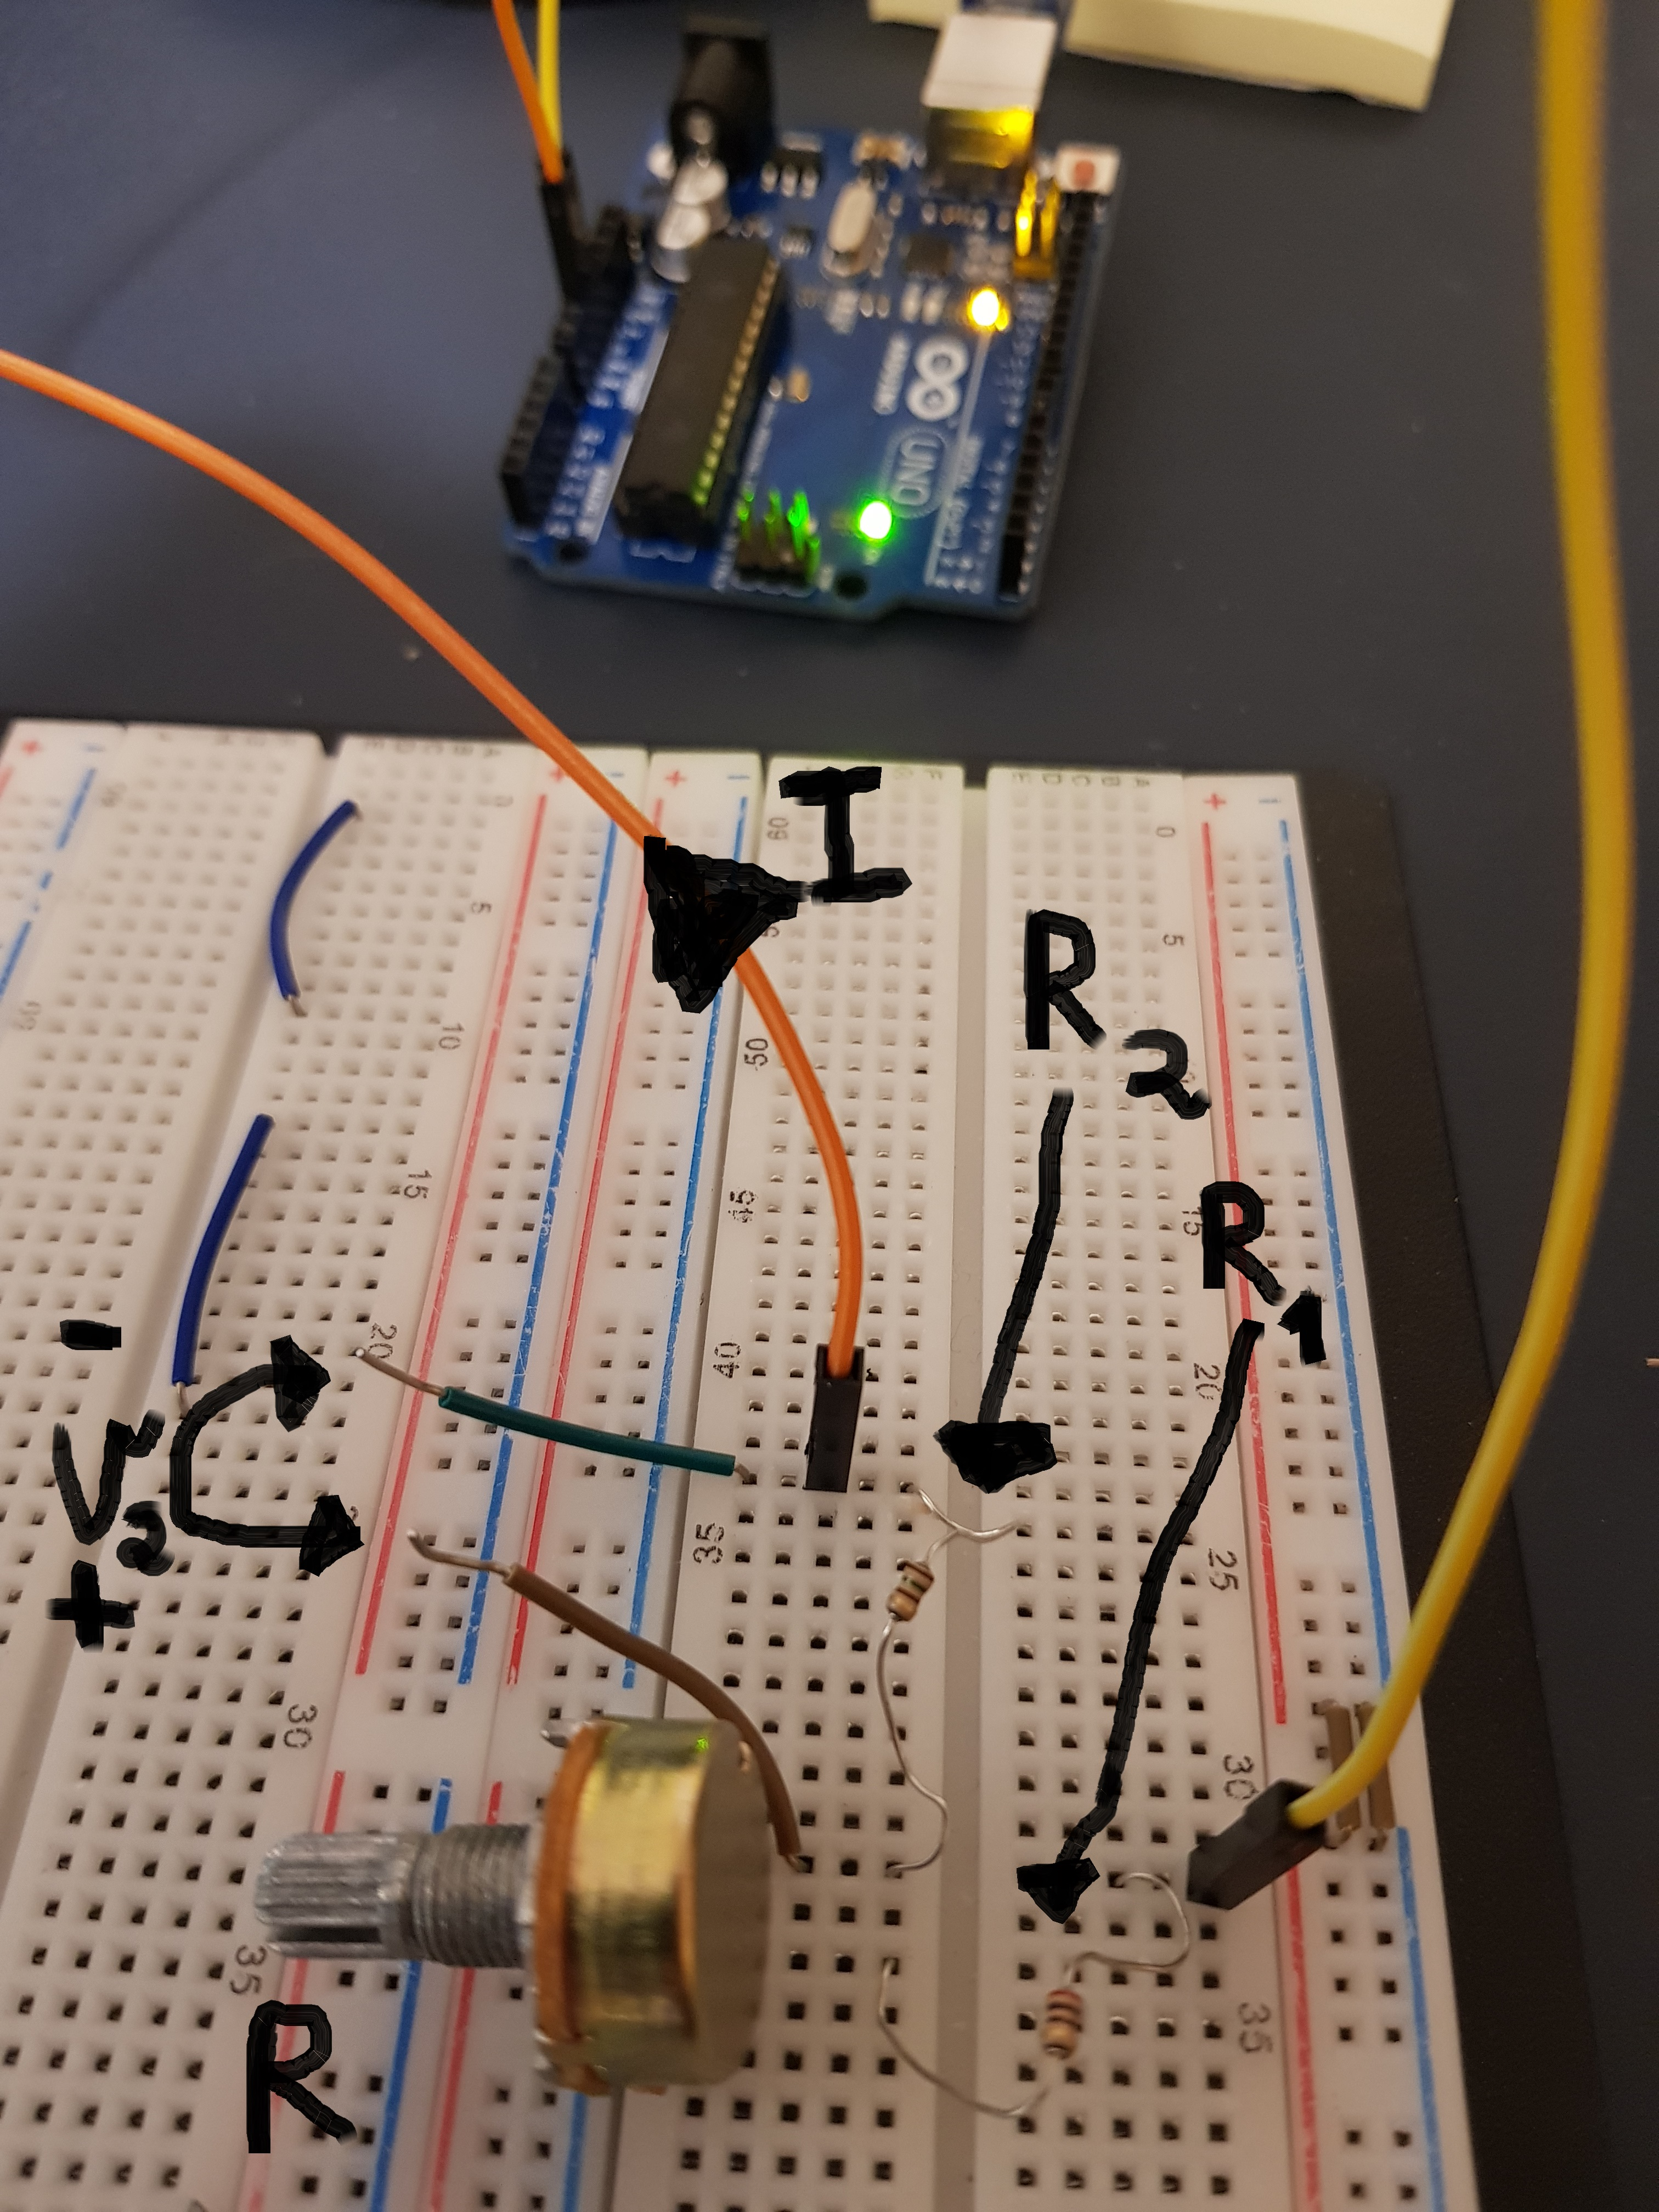
\includegraphics[width=0.6\textwidth]{realKrets}
    \caption{Reell krets av figur~\ref{fig:krets}}.
    \label{fig:realKrets}
\end{figure}

Det blir her brukt en spenningskilde $V=v_1=4,78V$. Likning~\ref{eq:reduceV} gir da at
\spliteq {
    & A_{1}: \quad v_{A_1} = V\cdot A_1 = 1,6969V \\
    & A_{2}: \quad v_{A_2} = V\cdot A_2 = 0,0674V
}\label{eq:realV2}
\newpage
Det gjøres målinger av spenningsfallet over $R_2$, ved forskjellige verdier av $R$. Oppførselen er vist på grafen til figur~\ref{fig:graph}.
\begin{figure}[htbp]
    \centering
    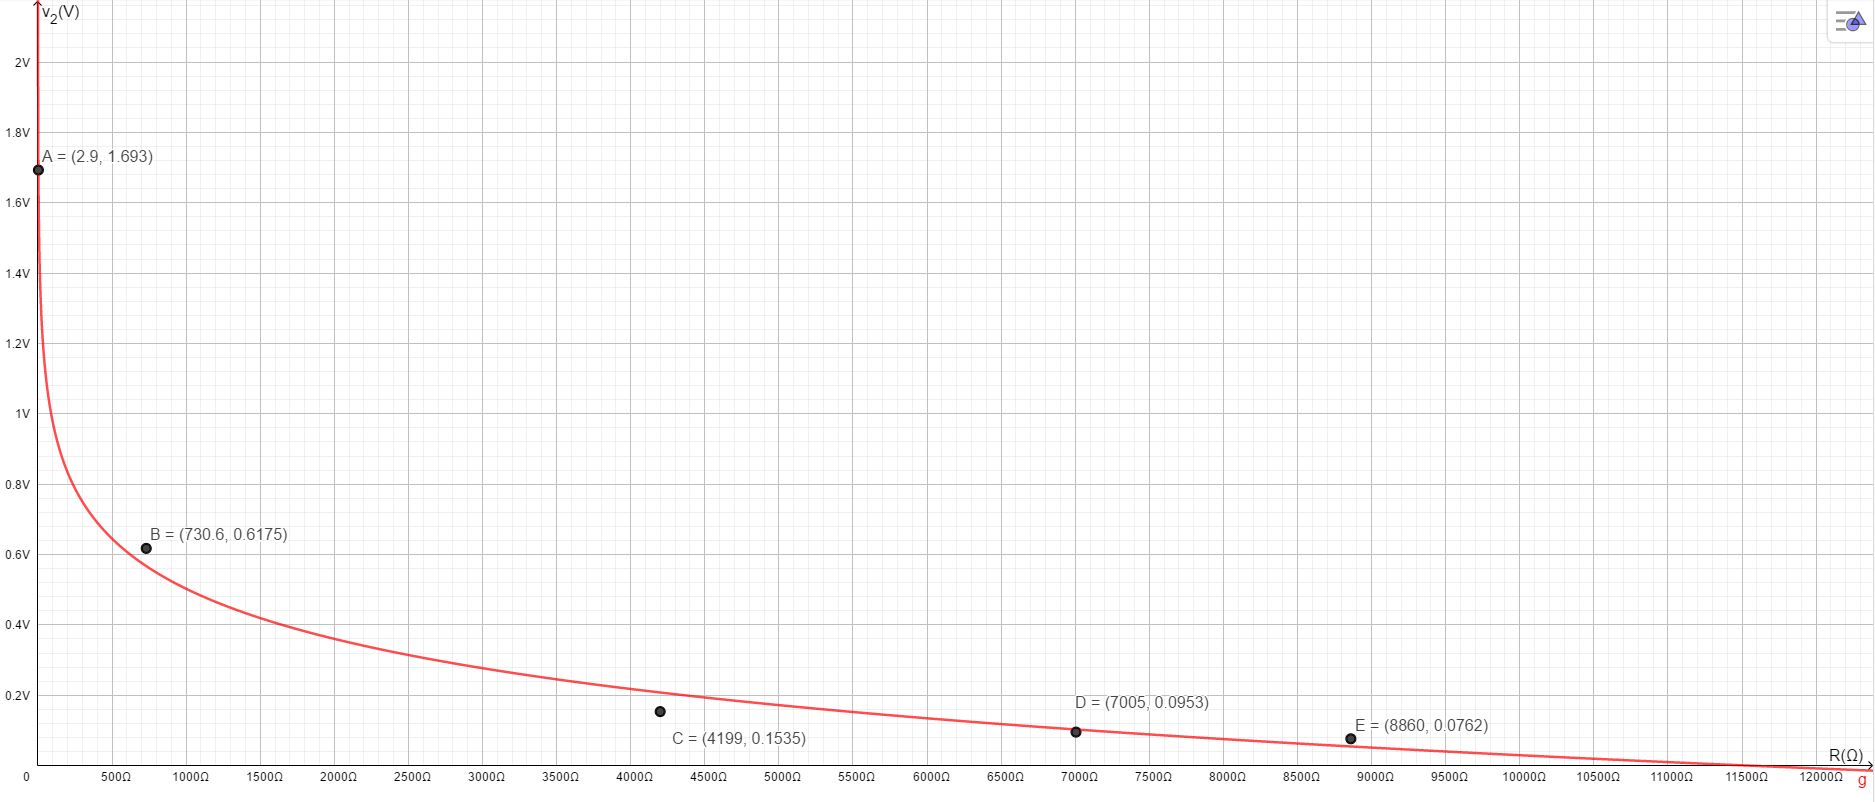
\includegraphics[width=1\textwidth]{graph}
    \caption{Oppførselen til $v_2$ når $R$ endres.}
    \label{fig:graph}
\end{figure}

Det første som er verdt å merke er at potensiometeret $R$ ikke kan nå $0\Omega$, men stopper ved $2,9\Omega$ og at den største verdien kun er $8,8k\Omega$. Dette vil gi avvik fra likning~\ref{eq: resistors}, der avviket til $v_A_1$ er $39mV$ og $v_A_2$ er $8,8mV$.
For å finne ut om avviket har en betydning for $A_1$ og $A_2$, så kan vi bruke likning~\ref{eq: amplitude} og konvertere til dB, slik at 
\spliteq {
   & A_{avvik 1} = -9dB - 20\cdot\log_{10}{\left(\frac{1.693V}{4.78V}\right)} = 0,015dB  \\
   & A_{avvik 2} = -37dB - 20\cdot\log_{10}{\left(\frac{0.0762V}{4.78V}\right)} = 1,05dB
}
 Verken $A_1$ eller $A_2$ er innenfor det gitte toleranseområdet fra seksjon~\ref{sec:innledning} på 0,1dB. En av årsakene til dette er at motstandene brukt i testingen har et avvik på $R_t\in\pm[0\Omega,5\Omega]$ fra motstandene som ble regnet ut i likning~\ref{eq: resistors}. \\
Det er også mulig å se på grafen over, at den ikke er linær, men nærmere en logaritmisk funksjon, som også vil bidra til ukorrekte verdier.
\\\\
Noe som er verdt å merke seg er at målingene er gjort ved likestrøm, som kan gi annerledes resultat fra vekselstrøm, men teorien som er lagt frem vil gjelde for begge.
\newpage
\section{Konklusjon}
\label{sec:konklusjon}
Det er brukt en av flere mulige metoder for å utvikle en nivåregulator som kan dempe et utgangssignal. Målet var å kunne dempe signalet innenfor et variabelt område med en toleranse på 0,1dB. Etter realiseringen av nivåregulatoren, så kom det frem at avviket ble større en godkjent toleranse, som blant annet skyldes at de realistiske komponentene ikke er nærme nok til de teoretiske beregningene. Skal resultatet forbedres, så må det eventuelt velges andre nedre- og øvre-grenser på $A$ eller bruke realistiske motstander med verdier nærmere den teoretiske modellen.

%Bibliografi: Legg til flere elementer ved å legge til flere \bibitem:--------
\phantomsection

\appendix
%Tillegg. Flere tillegg legges til ved å lage flere sections:-----------------
\section{Utledning av $R_1$ og $R_2$}\label{attach:resistors}

Gitt likning~\ref{eq: amplitude}, så har vi at
\spliteq {
    A = \frac{v_2}{v_1}
}
Fra figur~\ref{fig:krets}, som viser seriekobling av motstandene $R_1, R_2$ og $R$, så fremgår det at
\spliteq {
    A = \frac{R_2}{R_1 + R  + R_2}
}

Siden minimumsamplituden $A_1 \implies R = 0\Omega$ og maksimumsamplituden $A_2 \implies R = R_{max}$, så har vi likningsssytemet
\spliteq {
    A_1 = \frac{R_2}{R_1+R_2}\comma
    A_2 = \frac{R_2}{R_1+R_2+R_{max}}
}
der $R_1$ og $R_2$ er de ukjente. \\\\
Løsningen av likningssystemet gir oss at
\spliteq {
    R_1 = \frac{R_2(1-A_1)}{A_1} \comma
    R_2 = \frac{A_1A_2R_{max}}{A_1-A_2}
}


\end{document}